\documentclass{article}
\usepackage{graphicx}
\usepackage{algorithm}
\usepackage[noend]{algorithmic}
\usepackage{subfigure}
\usepackage{amssymb, amsmath, graphicx, charter, latexsym}
\usepackage{layouts}
\usepackage[letterpaper]{geometry}
\usepackage{enumerate}
\usepackage{epstopdf}
\usepackage{ragged2e}
%\usepackage{times}
\usepackage{mathtools}
%\usepackage[scaled]{helvet}
\usepackage{mathptmx}
\usepackage{verbatim}
\usepackage{listings}
\usepackage{siunitx}
\usepackage{booktabs}

\lstset{
basicstyle=\ttfamily,
}
\lstMakeShortInline|

\begin{document}

\title{\bf ECEN 689-- Real-Time Wireless Networks: Project 2\\ (Due on 4/1)}
\date{}
\author{%
Ping-Chun Hsieh\\
\texttt{lleyfede@tamu.edu}
\and
Tao Zhao\\
\texttt{alick@tamu.edu}
\and
Dongni Han\\
\texttt{handongni2015@tamu.edu}
}
\maketitle

\section*{Terminology}

In our report, we use ``server'' to denote the WiFi access point (AP), and
``client'' to denote the terminal device such as a mobile phone, a tablet, and
so on. Throughout our simulation, we let node $0$ be the server, and the other nodes be the clients. The basic time unit for packet transmission is called \emph{slot}, which should be greater than a round-trip time (RTT). For real-time traffic, we group an integer number (denoted by $T$) of slots into an \emph{interval}, which is the relative deadline of the packets. 

S-WiFi is the name of our application as well as our project. It stands for
Smart WiFi, or whatever you think it is.

%\section*{Simulation Setup}

\section*{Uplink Transmissions with PCF}
\label{section: uplink}
Throughout the report, we consider a wireless network of one AP and $N$ clients, where $N>1$. We consider uplink transmission with PCF from the clients to the AP. In PCF mode, the AP has full control over channel allocation. In the beginning of each interval, each client generates a random number of packets and waits for channel access that is fully controlled by the AP. Since the packets are generated and queued on the client's side, the AP needs to collect the queue information of the clients to make scheduling decisions. The baseline policy is described in Section \ref{section: baseline}.
\section{Baseline Policy}
\label{section: baseline}


\frenchspacing  Under the baseline policy, there are two phases in each interval. In the \emph{polling phase}, the AP collects the queue information by polling each client in a round-robin fashion. In the \emph{scheduling phase}, the AP schedules one of the clients based on the queue information and channel reliability.

\subsection{Polling Phase}
In the beginning of each interval, the AP gathers the queue information by sending \lstinline|SWiFi_POLL_NUM| packets to each client based on round-robin policy. Upon receiving the \lstinline|SWiFi_POLL_NUM|, the client will reply with a \lstinline|SWiFi_PKT_NUM_UL| packet which contains the queue information in the packet header. If either the transmission of \lstinline|SWiFi_POLL_NUM| or \lstinline|SWiFi_PKT_NUM_UL| fails, the AP will retransmit the \lstinline|SWiFi_POLL_NUM| packet again to the same client in the next slot. 
The polling phase ends when the AP receives all the queue information from the clients.

In the real-time scenario, the queue information is referred to as the number of packets generated in the current interval. On the other hand, for the non-real-time traffic, the queue information corresponds to the total number of packets received up to the present (denoted by $X_n$), which is used by the AP to obtain the real queue length of each client.    
%The AP will first send a POLL packet to the selected client. A client can only transmit its packet after it receives the POLL packet from the AP. This allows the AP to have full control over which client transmits. 

%Baseline policy: At the beginning of each interval, the AP asks each client, one by one, the number of packets that it generates. After this process, the AP also knows the number of packets at each client, and it can make the best decision.
\subsection{Scheduling Phase}
In each slot of the scheduling phase, the AP applies the Max-Weight policy, which schedules the client that maximizes the product of the queue length and the channel reliability. The AP sends a \lstinline|SWiFi_PKT_POLL_DATA| packet to the target client to provide access to the channel. When the scheduled client receives the data polling request, it will reply a packet of type \lstinline|SWiFi_PKT_DATA_UL| immediately to the AP. If the AP receives the data packet successfully, the AP will decrease the queue length by 1. If either the transmission of data polling or the data packet fails, the AP will stay with the same schedule in the next slot (suppose the next slot is not the end of the interval). Note that in the non-real-time scenario, in order to derive the real queue length of each client, the AP needs to keep track of the total number of received packets (denoted by $Y_n$) from each client $n$, and then calculates the queue length as $(X_n - Y_n)$ for each client $n$.

If the AP already receives all the packets available in the current interval, it will simply idle until the start of the next interval.

%Besides, we define four data types. 
     

\section{Implementation in NS-2}
\label{section: ns2}

Because there is no PCF functions available in 802.11 Mac module in ns-2, and we
prefer to make minimal changes to the 802.11 Mac implementation itself, we
implement the PCF functions with the baseline policy in the application layer,
where we define the \lstinline|hdr_swifi| packet header and the \lstinline|SWiFiAgent| class.

In the beginning of simulation, one node becomes the server AP by issuing the
\lstinline|server| command. For example,
\lstinline|$sw(0) server| makes the zeroth node the server.
Client registration is done by the \lstinline|register|
command. For instance, \lstinline|$sw_(0) register 1 0.5|
registers node 1 as a client with channel reliability $0.5$.%
\footnote{We use a lookup table to map the distance between the server and the
client to the channel reliability based on the result of reliability measurement
in project 1.}

\newcommand\CC{C\nolinebreak[4]\hspace{-.05em}\raisebox{0.3ex}{++}}

In the beginning of each interval, the server calls |boi|, which stands for
``beginning of interval'', to reset its internal state and packet counters.
Each client generates a random number of packets from a uniform distribution,
and uses the |pour| command to make it available from Tcl to \CC.

At each time slot, the server executes the \lstinline |poll| command.
Based on its state, it either sends a certain type of poll packet, or idle.
In the beginning of each interval, the server is in the |SWiFi_POLL_NUM| state,
and calls \lstinline |scheduleRoundRobin(false)| to find the next client
to poll the number of new packets
in the order of initial registration. Here |false| means
once all clients have been scheduled exactly once, no one will be scheduled
again, instead of scheduling from the first one repeatedly.
The server sends a |SWiFi_PKT_POLL_NUM| packet to the target client.

When the client receives the |SWiFi_PKT_POLL_NUM| packet, it replies a
|SWiFi_PKT_NUM_UL| packet with its number of packets in the packet header.
The number is the number
of newly generated packets in this interval for real-time traffic, while it is
the number of total generated packets up to now for non-real-time traffic.
When the server receives the packet, it acquires the number, and calculates the
queue length of the client. For real-time traffic, the queue length is the same
as the received number. For non-real-time traffic, the queue length is
equal to the received number minus the number of total delivered packets for
this client up to now.

After all clients have been polled for their numbers of packets, the server's
poll state goes into |SWiFi_POLL_DATA|, where actual data packets are polled.
Then, we need function \lstinline |scheduleMaxWeight| to implement maxweight policy. 

Besides, we define four packet types. 
\begin{table}[h!]
   \centering
   \caption{Packet types.}
   \label{tab:table3}
   \begin{tabular}{| l | l |}
      \hline
      Packet Type  &  Meaning\\ \hline
      \lstinline |SWiFi_PKT_POLL_NUM| & Poll number of packets in uplink\\ \hline 
      \lstinline |SWiFi_PKT_POLL_DATA|  & Poll data packet transmission in uplink\\ \hline 
      \lstinline |SWiFi_PKT_NUM_UL| & Packet in uplink that carries number of packets at client\\ \hline 
      \lstinline |SWiFi_PKT_DATA_UL| & Data packet in uplink (client to server)\\  
     \hline
   \end{tabular}
\end{table}
 
  
What's more, four poll states are defined below. 
\begin{table}[h!]
   \centering
   \caption{Poll states.}
   \label{tab:table4}
   \begin{tabular}{| l | l |}
      \hline
      Poll State  &  Meaning\\ \hline
      \lstinline |SWiFi_POLL_NONE| & Uninitialized \\ \hline 
      \lstinline |SWiFi_POLL_NUM|  & Poll the number of packets\\ \hline 
      \lstinline |SWiFi_POLL_DATA| & Poll a data packet\\ \hline 
      \lstinline |SWiFi_POLL_IDLE| & Idle\\  
     \hline
   \end{tabular}
\end{table}
     
\begin{figure}[htbp]
\centering
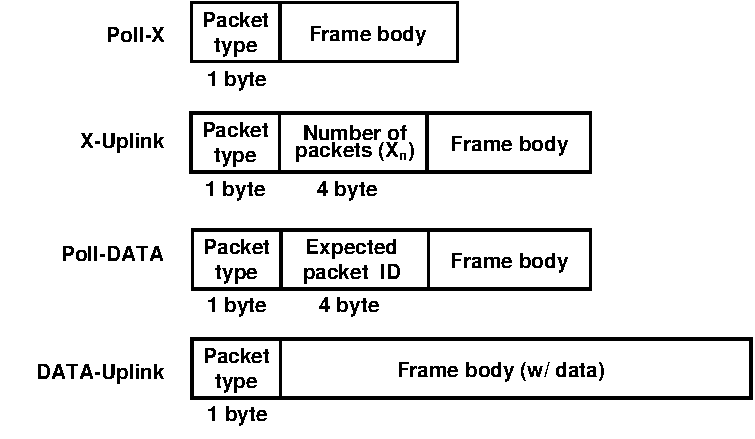
\includegraphics[scale=0.6]{header.pdf}
\caption{Packet Type}
\label{header}
\end{figure}

However, there are still some issues. Look at Figure \ref{discussion_1}, there is a possibility that AP Poll-X or a client poll X1 is not delivered successfully. Our method is retransmit Poll-X until the AP receives Xn. And we just set Xn = 0 if poll X does not deliver successfully. 

\begin{figure}[htbp]
\centering
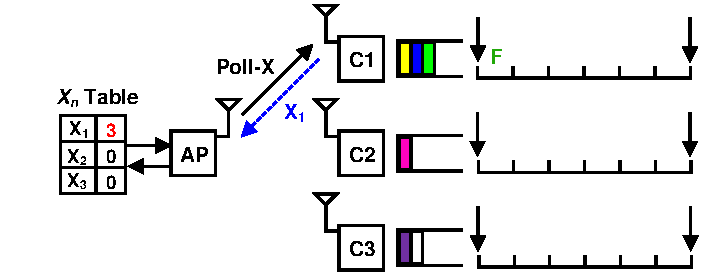
\includegraphics[scale=0.8]{discussion_1.pdf}
\caption{Issue 1}
\label{discussion_1}
\end{figure}

Look at Figure \ref{discussion_2}, how does a client know the DATA packet is delivered? Do we need an application-layer ACK for AP?  We put expected packet ID in Poll-DATA packets so that the client knows its last packet is delivered when AP asks its next packet. Thus, we needn't an application-layer "ACK" for AP. 

\begin{figure}[htbp]
\centering
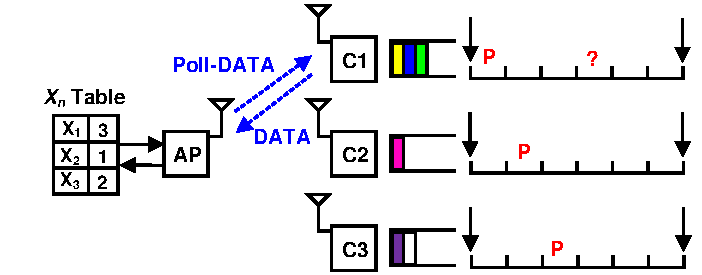
\includegraphics[scale=0.8]{discussion_2.pdf}
\caption{Issue 2}
\label{discussion_2}
\end{figure}

Look at Figure \ref{discussion_3}, what does "Xn" mean for non-real-time traffic? The answer is that the queue length equals total number of packets generated by a client minus total delivery of data packets from a client. So the max-weight policy chooses a client with the largest channel reliability times current queue length. 

\begin{figure}[htbp]
\centering
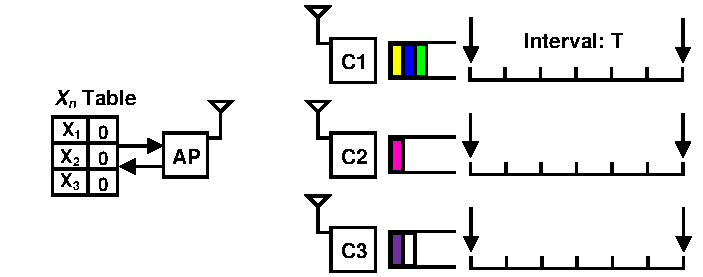
\includegraphics[scale=0.8]{discussion_3.pdf}
\caption{Issue 3}
\label{discussion_3}
\end{figure}


When the system captures a string called  \lstinline |poll|, tcl will print an error: only server AP can poll if it's not a server. If it's a server, the server(AP) will ask each client one by one using function \lstinline |scheduleRoundRobin| when the \lstinline |poll_state_| is  \lstinline |SWiFi_POLL_NUM|. And we set the packet type to \lstinline |SWiFi_PKT_POLL_NUM|, store current time and send the new packet. Otherwise, the server(AP) will use maxweight policy to schedule clients using function \lstinline |scheduleMaxWeight| when the \lstinline |poll_state_| is  \lstinline |SWiFi_POLL_DATA|. And we set the packet type to \lstinline |SWiFi_PKT_POLL_DATA|, store current time and send the new packet. Besides, there is one special condition that no more client is left in one interval (\lstinline |target_| is true). In this case, \lstinline |poll_state_| will be set to \lstinline |SWiFi_POLL_IDLE|.

When a client receives a packet type \lstinline |SWiFi_PKT_POLL_DATA| transmitted by a server, we save the old packet's send time, discard the old packet, create a new packet, set new send time and send this new packet to the server(AP). 
When a client receives a packet type \lstinline |SWiFi_PKT_POLL_NUM| transmitted by a server, we set the data type to \lstinline |SWiFi_PKT_NUM_UL| meaning that it is uplink packet with numbers of packets at client, set new send time and send this new packet to the server(AP).
When a server receivers  a packet type \lstinline |SWiFi_PKT_NUM_UL| transmitted by a client, the current queue length is equal to the number of data packets generated minus the number of data packets received. For real-time traffic, the current queue length is equal to the number of data packets generated.  

For Real-time traffic: At the beginning of each interval, we need clean queues of all clients cause we don't need store the queue length last interval. The current queue length just equals random number of packets at the beginning of each interval. If all packets miss its deadline, we just drop those packets.

For Non-real-time traffic:  If all packets miss its deadline, we don't drop those packets. We need store the queue length last interval. The current queue length is equal to total number of data packets generated by clients minus total number of delivery data packets from clients. 

We consider this system as a state machine according to Figure \ref{state machine}. But NS-2 doesn't provide a state machine. We just define some enum to define these states. 

\begin{figure}[htbp]
\centering
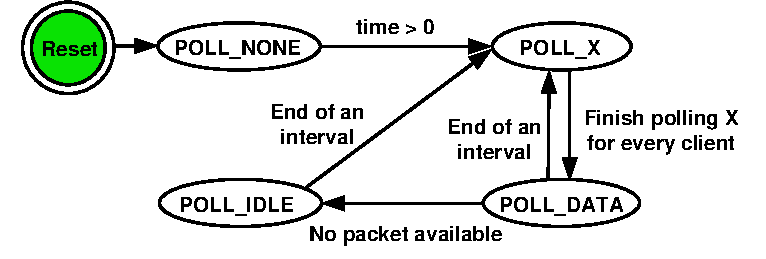
\includegraphics[scale=0.8]{state_machine.pdf}
\caption{State Machine}
\label{state machine}
\end{figure}


\section{Simulation Results}
\begin{table}[htbp]
\centering
    \caption{Parameters of the wireless channel.}
    \vspace{2mm}
    \begin{tabular}{ | l | l | }
    \hline
    Item & Value \\ \hline
    Path loss exponent & 2.0  \\ \hline
    Shadowing deviation & \SI{4.0}{dB} \\ \hline
    Reference distance & \SI{1.0}{m} \\
    \hline
\end{tabular}
\label{table: channel}
\end{table}
Throughout the simulation, we consider a fully-symmetric network with one AP and 2 clients. We use the shadowing module as the wireless channel. The parameters of the channel are summarized in Table \ref{table: channel}. The transmitter power level is \SI{1}{W}. The channel reliability can be changed by varying the distance between the AP and the clients. In our simulation, we set the distance between the AP and a client to be \SI{1}{m} when creating a reliable channel. For an unreliable channel with $p_n\approx 0.57$, the corresponding distance is \SI{1000}{m}. 

\begin{table}[htbp]
\centering
\caption{Parameters of the 802.11b MAC.}
    \vspace{2mm}
    \begin{tabular}{ | l | l | }
    \hline
    Item & Value \\ \hline
    Data rate & \SI{11}{Mb/s}  \\ \hline
    Basic rate & \SI{1}{Mb/s}  \\ \hline
    PLCP data rate & \SI{1}{Mb/s}  \\ \hline 
    Preamble length & \SI{144}{bits} \\ \hline
    Slot time & \SI{20}{\mu s} \\ \hline
    SIFS & \SI{10}{\mu s} \\
    \hline
\end{tabular}
\label{table: mac}
\end{table}

For the medium access control (MAC) layer, we use the 802.11 module built in ns-2. Following the IEEE 802.11b standard, the MAC layer parameters are chosen as in Table \ref{table: mac}. Besides, the automatic retry function built in 802.11 is disabled, i.e. \lstinline|ShortRetryLimit_| and \lstinline|LongRetryLimit_| are set to be 0 in the Tcl domain, to avoid channel congestion due to uncontrollable retransmission in the MAC layer.

Since ns-2 has no PCF module, we mimic PCF in the application layer. Throughout the simulation, a slot is chosen to be $\SI{10}{ms}$, which is much longer than a RTT ($\approx\SI{1.63}{ms}$), to provide enough margin for packet delivery. We consider random packet arrivals. The number of packets generated in an interval follows discrete uniform distribution that ranges between 0 and $N_{max}$. 


\label{section: simulation}
\subsection{Network Capacity}
We first study the network capacity with different packet generation rates under the baseline policy. Let $T=10$ and the channels be reliable, i.e. $p_1 = p_2 = 1$. We measure the average network throughput (denoted by $\bar{R}$) with different $N_{max}$.

In the non-real-time scenario, Figure \ref{nonrealtime_throughput_randmax} shows the system throughput for $N_{max}$ between 1 and 12. We can see that the maximum achievable throughput is 8, less than $T$. This is because the AP has to collect the queue information in the polling phase, which lasts for 2 slots in every interval. Therefore, polling indeed reduces the network capacity. Moreover, the dashed line shows the expected network throughput if there is no randomness in packet generation. Thus, for non-real-time traffic, randomness in packet generation does not affect the network throughput.
\begin{figure}[htbp]
\centering
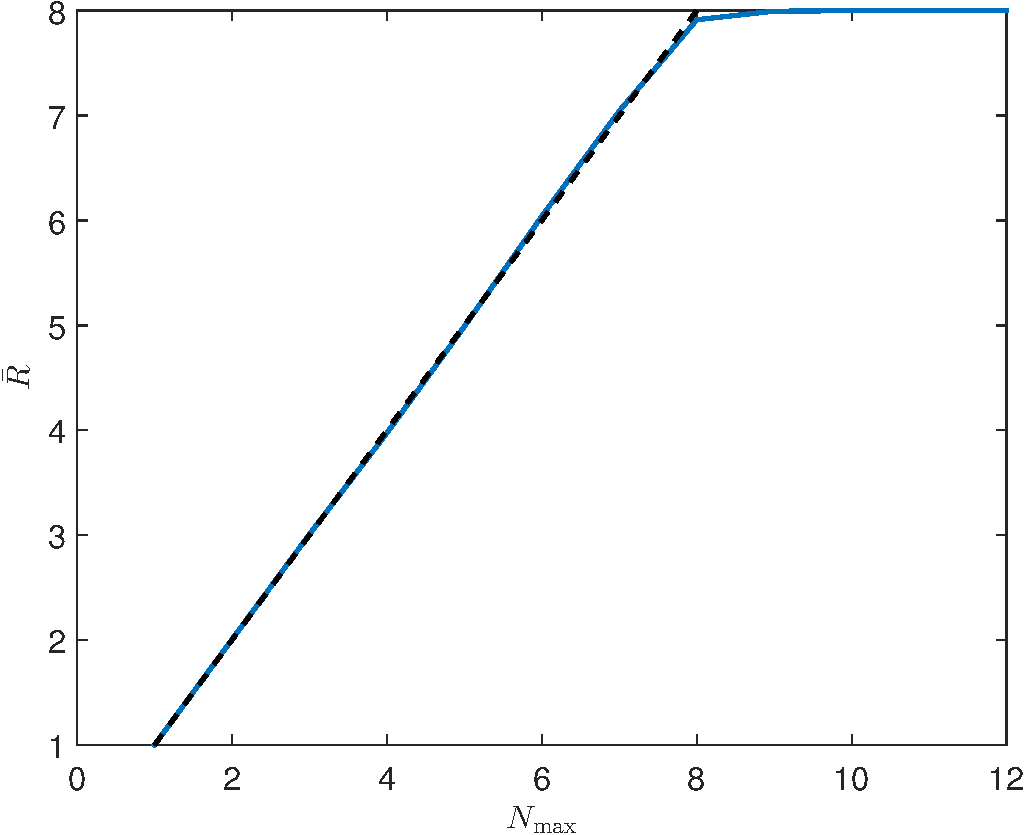
\includegraphics[scale=0.5]{nonrealtime_throughput_randmax.pdf}
\caption{Network throughput versus $N_{max}$ with non-real-time traffic}
\label{nonrealtime_throughput_randmax}
\end{figure}

For real-time traffic, the network throughput is shown in Figure \ref{realtime_throughput_randmax}. Compared to the non-real-time case, the network throughput with real-time traffic is smaller when $N_{max}\geq 5$. This is because packets may expire when the total packets generated in an interval is larger than 8, which is the length of the scheduling phase. Therefore, in addition to polling overhead, packet deadline can further reduce the network throughput. 

\begin{figure}[htbp]
\centering
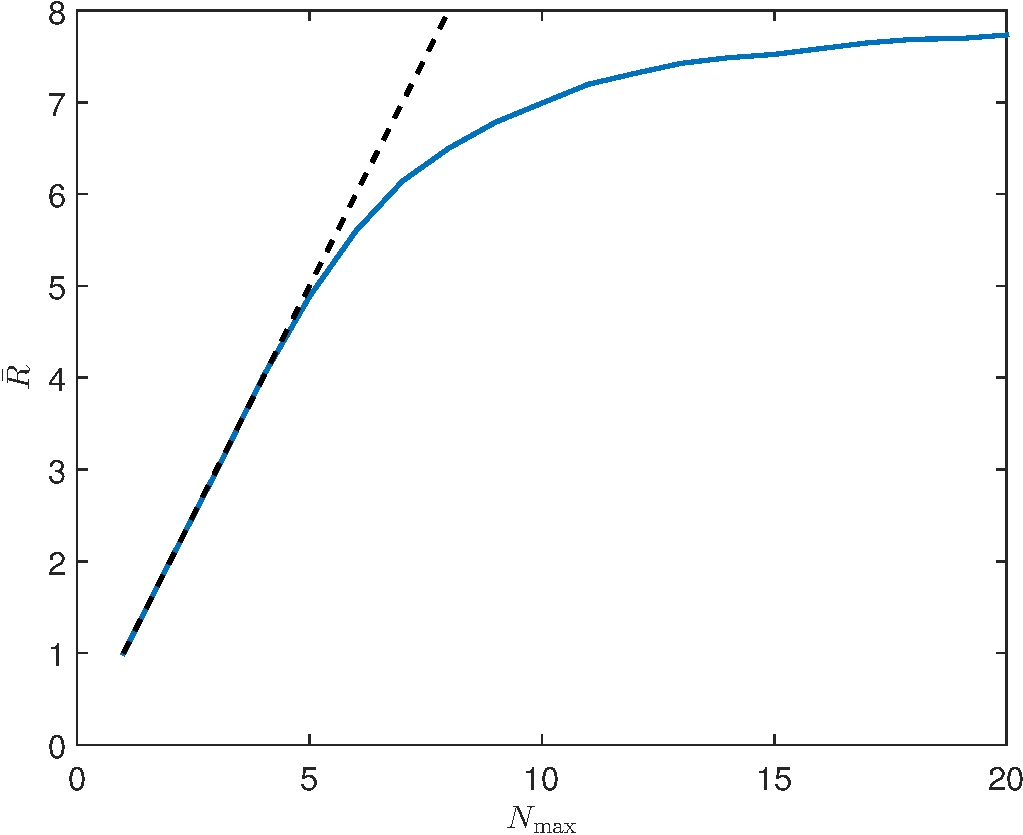
\includegraphics[scale=0.5]{realtime_throughput_randmax.pdf}
\caption{Network throughput versus $N_{max}$ with real-time traffic}
\label{realtime_throughput_randmax}
\end{figure}

\subsection{Choice of Interval Length}
We study the how the choice of $T$ affects the network throughput. Choose $N_{max}=2$ and $p_1 = p_2 = 0.57$. Figure \ref{nonrealtime_throughput_T} shows the network throughput with different interval length in the non-real-time scenario. The total throughput is very low when $T=4$ because the polling overhead is particularly significant for small $T$. Moreover, since larger $T$ implies more available slots to the scheduling phase, the system throughput should increase with interval length. 

%For non-real-time traffic, according to , T ranges from 4 to 16. We can conclude that interval should be long enough to guarantee deliveries. If interval is too short, AP will not have enough time slots to poll data to clients. 

\begin{figure}[htbp]
\centering
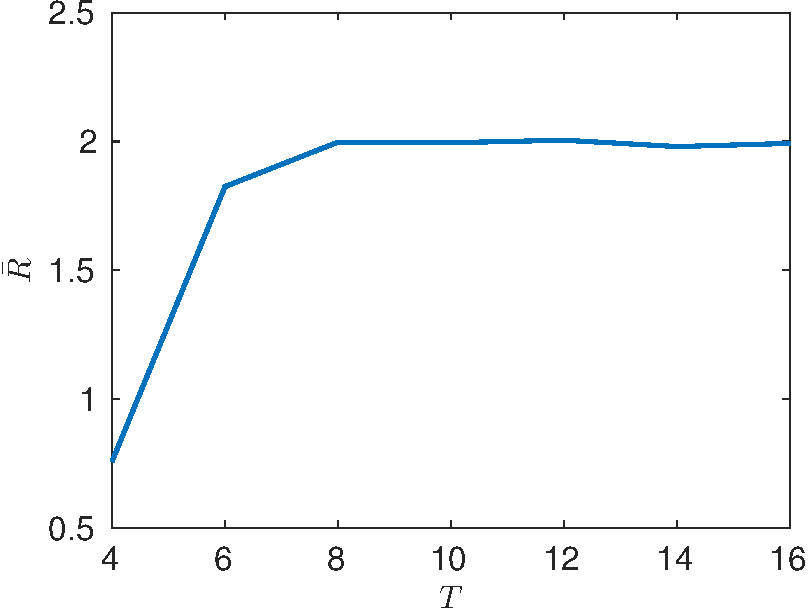
\includegraphics[scale=0.7]{nonrealtime_throughput_T.pdf}
\caption{Network throughput versus interval length with non-real-time traffic.}
\label{nonrealtime_throughput_T}
\end{figure}

Figure \ref{realtime_throughput_T} shows the network throughput with different interval length with real-time traffic. Compared to the non-real-time case, the throughput with real-time traffic is even lower due to possible packet expiration. In other words, real-time traffic requires larger $T$ so that the effect of the expired packets can be mitigated. Besides, Figure \ref{realtime_throughput_T} serves as a useful reference for system design. For example, suppose both clients require a delivery ratio of 0.6. From Figure \ref{realtime_throughput_T}, we need to choose $T\geq 8$ to meet the requirement. 

\begin{figure}[htbp]
\centering
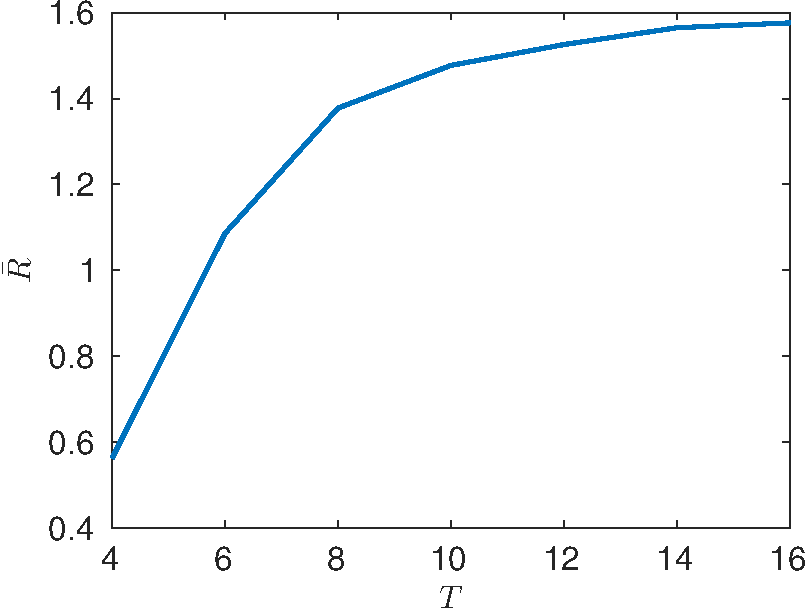
\includegraphics[scale=0.7]{realtime_throughput_T.pdf}
\caption{Network throughput versus interval length with real-time traffic.}
\label{realtime_throughput_T}
\end{figure}

\subsection{Network Size and Polling Overhead}
\begin{figure}[htbp]
\centering
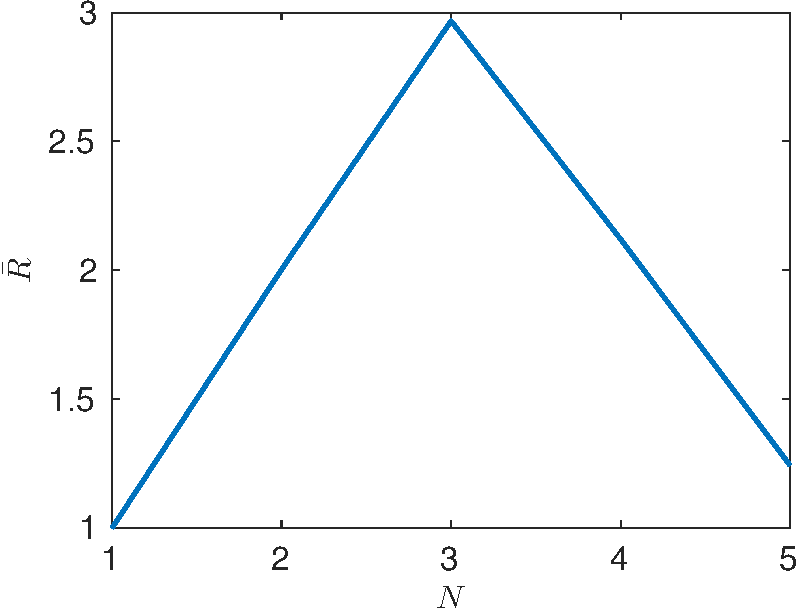
\includegraphics[scale=0.7]{nonrealtime_throughput_N.pdf}
\caption{Network throughput versus network size with non-real-time traffic.}
\label{nonrealtime_throughput_N}
\end{figure}

%For real-time traffic, according to Figure \ref{realtime_throughput_N}, N ranges from 1 to 5. We can conclude that channel performance is even worse compared with non-real-time traffic and it also degrades with more clients. The reason is that packets will expire if they miss its deadline.  

\begin{figure}[htbp]
\centering
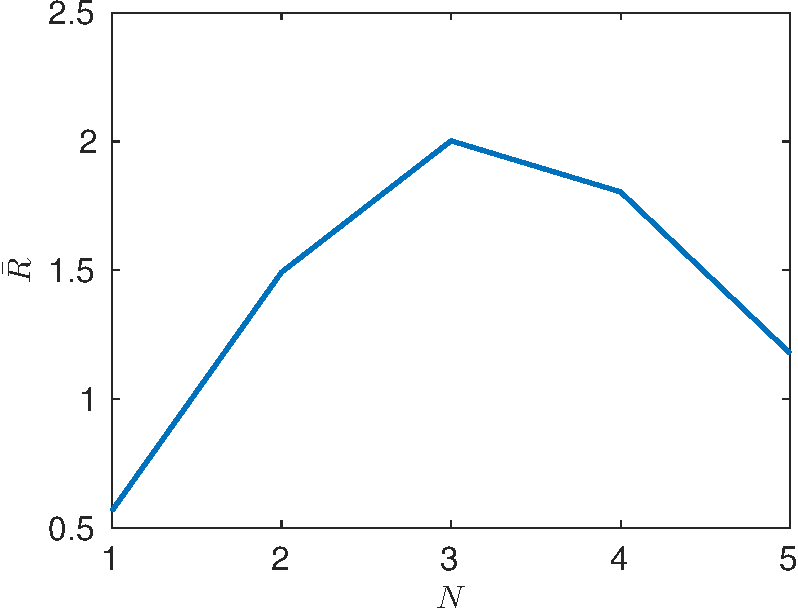
\includegraphics[scale=0.7]{realtime_throughput_N.pdf}
\caption{Network throughput versus network size with real-time traffic.}
\label{realtime_throughput_N}
\end{figure}
We study the effect of network size on the polling overhead. Let $T = 10$, $N_{max}=2$, and channel reliability $p_1 = p_2 = 0.57$. Figure \ref{nonrealtime_throughput_N} shows the network throughput with non-real-traffic traffic for different network size. When $K$ grows from 1 to 3, the total throughput increases since the total traffic is not saturated yet. As $K$ exceeds 3, the network throughput drops significantly because the polling phase takes most of the time in an interval. Figure \ref{realtime_throughput_N} shows a similar pattern for the real-time case. 

In both scenarios, the network performance degrades severely with more clients. Hence, the baseline policy is not suitable for large networks due to the polling overhead. 
%For non-real-time traffic, according to , N ranges from 1 to 5. 



\section{Conclusion}
The baseline policy employs a simple polling scheme to collect queue information of the clients. Accordingly, the AP can be work-conserving in the scheduling phase. However, the channel utilization for data packets can be low due to the polling overhead. The overhead can degrade the network performance even more severely when the number of clients is large or the interval length is small. To mitigate this effect, we definitely need a smarter policy to accommodate uplink transmission with PCF.

\end{document}
